\documentclass[a4paper,12pt]{report}

\usepackage{graphicx}

\setlength {\textheight}{247mm}
\setlength {\textwidth}{168mm}
\setlength {\oddsidemargin}{0cm}
\setlength {\evensidemargin}{0cm}
\setlength {\headsep}{0cm}
\setlength {\headheight}{0cm}
\setlength {\topmargin}{0cm}
\setlength {\leftmargin}{0cm}
\setlength {\unitlength}{1cm}
\setlength {\parindent}{0cm}

\title{Implementation of a dynamic invocation interface for AdaBroker}
\author{S\'ebastien Ponce}
\date{\today}

\begin{document}

\maketitle

\begin {abstract}
\paragraph{}The problem you have each time you try to write a documentation is the following : 
how to make it interesting for non specialists without
boring the specialists ? To solve it, we choose to use the same structure as John Barnes did in his ``Programming in ADA 95''.
\paragraph{}So the first part is dedicated to non specialists who need a general presentation of the CORBA concepts. It first
presents what CORBA is (Common Object Request Broker Architecture), then what AdaBroker is (a free, GPL released Ada ORB).
 At last, it describes
the two invocation mechanisms provided in CORBA : the static one and the dynamic one.
\paragraph{}The second part is more specialized and describes in details the implementation of the
Dynamic Invocation Interface in the AdaBroker product. You can find there explanations on all the types
used in the DII (Any, TypeCode, NamedValue, NVList) as well as explanations on the way to build a request and to call the ORB on it.
\end{abstract}

\tableofcontents

%%%%%%%%%%%%%%%%%%%%%%%%%%%%
%%%  Make it simple stupid
%%%%%%%%%%%%%%%%%%%%%%%%%%%%%
\part{Keep it simple stupid}

\paragraph{}This first part intends to be readable by everyone (maybe everyone knowing Ada for the last two chapters).
 It briefly presents CORBA and the AdaBroker 
product before explaining the way operations are invoked in AdaBroker, both statically and dynamically.
\paragraph{}Reading this part, you should already be able to build a simple application using CORBA and AdaBroker. If you need more 
technical information or if you are interested in the way AdaBroker is built, please refer to the next part.

%%%%%  Overview of CORBA
%%%%%%%%%%%%%%%%%%%%%%%%%
\chapter{Overview of CORBA}

\paragraph{}You'll find here a general introduction to CORBA as well as an explanation of the way it works globally.
If you already know something on CORBA, just skip this chapter.

%%%  OMG
\section{The OMG}
\paragraph{}The {\bf O}bject {\bf M}anagement {\bf G}roup is a consortium created in 1989 
that puts together more than 850 actors of the new economy :
contructors like Sun or IBM, software sellers like Netscape, Inprise or Visigenic, users like Boeing or Alcatel and institutions or
universities like NASA, INRIA, LIFL. The goal of this group is to create standards for the integration of heterogeneous applications
on distributed systems using object oriented technologies. The key concepts are thus reusability, interoperability and portability
of software components.
\paragraph{}The key element of the OMG vision is CORBA : {\bf C}ommon {\bf O}bject {\bf R}equest {\bf B}roker {\bf A}rchitecture.
It is an object oriented middleware that provides an execution support hiding the technical levels of a distributed system (operating
system, processor and network). It deals with all the communications between software components building heterogeneous distributed
applications.
\paragraph{}

%%%  Client-server model
\section{a Client - Server architecture}
\paragraph{}The CORBA model is based on a classical client-server architecture. There is thus two types of applications using CORBA : clients and servers (even if you can be both at the same time). The servers provide some functionnalities through objects and methods on them and the client can use them remotely through the CORBA Bus. The figure \ref{fig:CSModel} page \pageref{fig:CSModel} provides a schema of the mechanism.
\begin{figure}
\label{fig:CSModel}
\begin{center}
\includegraphics[angle=270,scale=0.5]{client-server_model.ps}
\caption{Client-Server Model}
\end{center}
\end{figure}


%%%  Adabroker
%%%%%%%%%%%%%%%%%%%%%
\chapter{Overview of AdaBroker}
\paragraph{}You'll find here a general introduction to AdaBroker, a GPL released Ada ORB for CORBA.

\section{What it is}
\paragraph{}AdaBroker is an Ada ORB for CORBA. It all began with a student project at the ENST (Ecole Nationale Sup�rieure des T�l�coms) in Paris, France in Januar 1999. The first version (beta 0.8) was released in the summer 99 and already provided most of the existing CORBA fetures. It was mostly based on external component since it used the Sun front-end for the parsing of Idl in the Idl to Ada compiler and the OmniORB ORB.
\paragraph{}The first major work for the AdaBroker team was to rewrite all the components in Ada in order to provide an independant, full Ada software. This was achieved in version 1pre1, released in April 2000. The two main components of the AdaBroker software are now :
\begin{itemize}
\item {\bf idlac} as idl to Ada compiler, full written in Ada by the AdaBroker team
\item {\bf broca} as ORB, also full written in Ada by the AdaBroker team
\end{itemize}
\paragraph{}In this 1pre1 version, the features were still the same :
\begin{itemize}
\item full static invocation mechanism
\item management of exceptions
\item management of forward declarations (to allow recursive definitions)
\item management of multiple inheritance in Idl
\end{itemize}
Some components were missing to provide a full ORB :
\begin{itemize}
\item Dynamic invocation (both client and server part)
\item management of values
\item interface repository
\item the major services  cosNaming, cosEvent, cosTime...
\end{itemize}
Most of these components are currently under developpement and the next release (1pre3 or next one) will provide dynamic invocation (client part, an interface repository, the management of values and some services. This is the purpose of this document to describe at least the dynamic invocation mechanism on the client side.

\section{How to get it}
You just have to go to http://adabroker.eu.org. You can download the soft there and have some information concerning the mailing lists and current releases. This site is hosted by Ada France.

%%% Static invocation Mechanism
%%%%%%%%%%%%%%%%%%%%%%%%%%%%%%%%%%
\chapter{The static invocation mechanism}
\label{SIM}
\paragraph{}We'll present the static invocation mechanism through the most simple example you can think of : the echoString example.
Just try here to imagine what string we could use to test it (beginning by ``Hello'')... However, each time this example does not fit
to describe the general case, we'll mention it and explain the whole thing.
\paragraph{}So here is the IDL specification of this example :
\begin{verbatim}
interface Echo {
  string echoString (in string Mesg);
};
\end{verbatim}

\paragraph{}The normal (and static) way to build a client-server application on this IDL interface consists in two steps :
first building the server and then the client.

%%%%%%  Building a Server
\section{Building a server}
\paragraph{}The server itself has two main parts : an implementation, which is the code that effectively 
does the job, here echoing a string, and a skeleton which is an interface between your implementation and the ORB, allowing the ORB to 
call your code.
\paragraph{}Both parts can be generated automatically using an IDL to Ada compiler. Here we use {\it idlac}, provided in the 
AdaBroker package. The skeleton can be fully generated whereas the implementation is just a framework you'll have to fill in.

Note that the implementation is not generated by default, in order not to remove some already filled in files. You have to use the '-i' flag
to generate it.

\subsection{Implementation}
\paragraph{}Let's have a look at the implementation files first. Nothing surprising there. Here is the spec :
\begin{verbatim}
package Echo.Impl is

   type Object is new PortableServer.Servant_Base with null record;

   function echoString (Self : access Object;
                        Mesg : in CORBA.String)
                        return CORBA.String;
end Echo.Impl;
\end{verbatim}
and here is the empty implementation :
\begin{verbatim}
package body Echo.Impl is

   function echoString (Self : access Object;
                        Mesg : in CORBA.String)
                        return CORBA.String is
      Result : CORBA.String;
   begin
      --  Insert implementation of echoString
      return Result;
   end echoString;

end Echo.Impl;
\end{verbatim}
In our case, the implementation is easy to build, we just have to insert ``\texttt{Result := Mesg;}'' where indicated.

\subsection{Skeleton}
\paragraph{}As I already mentionned it, the skeleton files (echo-skel.ads/adb) are fully generated by {\it idlac}. However, it is interesting to have a look at them in order to understand the invocation mechanism.
\paragraph{}Here is the interesting part of echo\_skel.adb :
\begin{verbatim}
   procedure GIOP_Dispatch
     (Obj : PortableServer.Servant;
      Operation : String;
      Request_Id : CORBA.Unsigned_Long;
      Response_Expected : CORBA.Boolean;
      Request_Buffer : access Broca.Buffers.Buffer_Type;
      Reply_Buffer   : access Broca.Buffers.Buffer_Type) is
   begin
      if Operation = "echoString" then
        (...)
         declare
            IDL_Mesg : CORBA.String;
            Return_U : CORBA.String;
         begin
            --  Unmarshall in and inout arguments
            IDL_Mesg := Unmarshall (Request_Buffer);
            begin
               --  Call implementation
               Return_U := Echo.Impl.echoString (Object_Ptr (Obj), IDL_Mesg);
            end;
            (...)
            --  Marshall return value
            Marshall (Reply_Buffer, Return_U);
            return;
         end;
      end if;
      Broca.Exceptions.Raise_Bad_Operation;
   end GIOP_Dispatch;
\end{verbatim}
\paragraph{}This method is actually called by the ORB each time there is a request on the echo object. The only significant arguments 
for us are \texttt{Operation} and the two buffers : \texttt{Request\_Buffer} and \texttt{Reply\_Buffer}. 

What this method does is 
simply looking at the operation name contained by \texttt{Operation}, getting the arguments of this operation from the 
\texttt{Request\_Buffer}, calling the actual implementation of the operation with these arguments (in echo.impl)
 and puting the result in the \texttt{Reply\_Buffer}.

\paragraph{}There could be some changes if you don't use exactly the same example :
\begin{itemize}
\item{}In case another method were defined on the echo object, you would have another \texttt{if Operation = ... then ... end if;} 
block for this method. Each block is dealing with a single method and the end of the \texttt{GIOP\_Dispatch} method is only reached when none of
the provided methods fits. In this case, an exception is raised. 
\item{}In case you had some out or inout arguments in your method, their return value would have been put
in the \texttt{Reply\_Buffer} with (actually in place of) the result.
\end{itemize}

%%%%%%  Building a Client
\section{Building a client}
We are here in the position of the user, that has just discovered the unbelievable power of the echo object and wants to use it remotely
in his application. Once more, there is two main parts in the code we'll need. The first part is the client application and the second one
a kind of proxy called {\it stub} being able to talk with the ORB and make it
execute remotely the method (possibly in an other langage, on an other architecture).

\subsection{A proxy to the ORB}

\paragraph{}This ``proxy'' is provided by the echo.ads and echo.adb files. Here is the main code of echo.adb :
\begin{verbatim}
package Echo is
   type Ref is new CORBA.Object.Ref with null record;

   function echoString (Self : in Ref;
                        Mesg : in CORBA.String)
                        return CORBA.String;
   (...)
end Echo;
\end{verbatim}

\paragraph{}We found here the definition of the echo object and the \texttt{echoString} method the client is interested in.
Here is the implementation of the \texttt{echoString} method in echo.adb :
\begin{verbatim}
   function echoString (Self : in Ref;
                        Mesg : in CORBA.String)
                        return CORBA.String is
      Handler_U : Broca.GIOP.Request_Handler;
      Send_Request_Result_U : Broca.GIOP.Send_Request_Result_Type;
      Return_U : CORBA.String;
   begin
      (...)
      loop
         --  Create a buffer and marshall the operation name
         Broca.GIOP.Send_Request_Marshall (Handler_U,
                                           Broca.Object.Object_Ptr (Get (Self)),
                                           True,
                                           echoString_Operation);

         --  Marshall in and inout arguments for the operation
         Marshall (Handler_U.Buffer'Access, Mesg);

         --  Send a request to the ORB
         Broca.GIOP.Send_Request_Send (Handler_U, 
                                       Broca.Object.Object_Ptr (Get (Self)),
                                       True,
                                       Send_Request_Result_U);

         --  Unmarshall return value.
         case Send_Request_Result_U is
            when Broca.GIOP.Sr_Reply =>
               Return_U := Unmarshall (Handler_U.Buffer'Access);
               Broca.GIOP.Release (Handler_U);
               return Return_U;
            (...)
         end case;
      end loop;
   end echoString;
\end{verbatim}

\paragraph{}The way it works is really simple : it creates a buffer where it marshalls (understand puts) the operation name and arguments,
then it calls the ORB giving this buffer to it and at last, it gets back the result.

You could find some modifications with other examples :
\begin{itemize}
\item{}If there was another method in echo, we'd have two generated methods, each calling the ORB with its own name and arguments.
\item{}If a method had out or inout arguments, we could get back their value from the same buffer where we got back the result.
\end{itemize}

\subsection{A client}
\paragraph{}The client is very simple to write since the invocation of the \texttt{echoString} method looks like as if it were local.
\begin{verbatim}
procedure Client is
   Sent_Msg, Rcvd_Msg, IOR : CORBA.String;
   myecho : Echo.Ref;
begin
  (...)
   --  transforms the Ada string into CORBA.String
   IOR := CORBA.To_CORBA_String (Ada.Command_Line.Argument (1));

   --  gets a reference on the server we want to use
   CORBA.ORB.String_To_Object (IOR, myecho);

   --  actual call to the method, through the ORB
   Sent_Msg := CORBA.To_CORBA_String (Standard.String'("Hello Static World !"));
   Rcvd_Msg := Echo.echoString (myecho, Sent_Msg);
   (...)
end Client;
\end{verbatim}

\paragraph{}Nothing to add on this section.

%%%%% What was static
\section{Conclusion : how was it static ?}
\paragraph{}Or what could be dynamic ?

\paragraph{}We saw through this example the absolute necessity for both the client and the server to compile the IDL interface through
an IDL compiler such as {\it idlac}. If you don't have it, you cannot call the ORB on the client side, and you cannot be called on the
server side. This implies that both client and server are very dependant on the IDL compiler (if this one changes, you'll have to change
your code) and on the IDL interface (you have to know all of it). That's what is considered as static in the whole thing.

\paragraph{}On the other hand, we would call dynamic an invocation that won't use the IDL compiler and will allow one client to adapt
to the server, discovering what methods it has and what kind of arguments it needs before calling it. That's exactly what the DII
(Dynamic Invocation Interface) proposes.

\paragraph{}Appart from these considerations on static/dynamic calls, did you notice that all the invocations to the ORB, in the client
part, were blocking ? That will be another feature of the dynamic invocation : the possibility to place asynchronous calls.

%%%% DII
%%%%%%%%%%%%%%%%
\chapter{The dynamic invocation mechanism}

\paragraph{}In the previous chapter, we saw all the mechanism of the static invocation mechanism and its limitations.
We present here the solution to these limitations : the dynamic invocation mechanism.

\paragraph{}The Dynamic Invocation Mechanism is supported on the client side by the Dynamic Invocation Interface. The idea here is to write a
kind of generic proxy that would be used for every existing object, instead of having one proxy per object. This proxy would be
able to marshall the operation name and arguments exactly in the same way as a dedicated proxy, so that the ORB and the server
will never know if the invocation was dynamic or not.

\paragraph{}In order to write such a generic proxy, you'll need some way of passing generic arguments to it. It means you need 
a self-describing type that is able to encapsulate any given value. This type is called \texttt{Any}; it is associated with the
\texttt{TypeCode} type used to describe a value type.

\paragraph{}Giving these generic type and a generic proxy, all works fine. Lets look further in all this, using the same example 
we used in chapter \ref{SIM}.

%%% The generic Proxy
\section{The generic proxy}
The generic proxy is provided through the {\it CORBA.Request} package described in the OMG specifications by this Ada specification :
\begin{verbatim}
package CORBA.Request is

   type Object is private;

   procedure Add_Arg
     (Self      : in out Object;
      Arg_Type  : in     CORBA.TypeCode.Object;
      Value     : in     System.Address;
      Len       : in     Long;
      Arg_Flags : in     Flags);
   procedure Add_Arg
     (Self : in out Object;
      Arg  : in     NamedValue);

   procedure Invoke
     (Self         : in out Object;
      Invoke_Flags : in     Flags  := 0);

   procedure Delete (Self : in out Object);

   procedure Send
     (Self         : in out Object;
      Invoke_Flags : in     Flags  := 0);

   procedure Get_Response
     (Self         : in out Object;
      Invoke_Flags : in     Flags  := 0);

   function Poll_Response (Self : in Object) return Boolean;

end CORBA.Request;
\end{verbatim}

\paragraph{}Even if this package does not look like what we had in the proxies of the static invocation, it has exactly the same
functions (and even a bit more). All the idea is to build a {\it Request} object containing all what is needed for the invocation
(basically the operation name and arguments) and to call the {\it invoke} or {\it send} method on this request
to make the actual call to the ORB.

\paragraph{}The only method that allows a user to create a new request is not in the {\it Request} package but in {\it CORBA.Object}.
 Its ada specification is the following :
\begin{verbatim}
   procedure Create_Request
     (Self      : in     Ref;
      Ctx       : in     CORBA.Context.Ref;
      Operation : in     Identifier;
      Arg_List  : in     CORBA.NVList.Ref;
      Result    : in out NamedValue;
      Request   :    out CORBA.Request.Object;
      Req_Flags : in     Flags);
\end{verbatim}

\paragraph{}Lets explain the use of all these methods :
\begin{itemize}

\item{\bf Create\_Request} This method takes as parameters all what is needed to make the call to the ORB :
\begin{itemize}
\item{\it Self} is a reference to the object to be called. In our case, an {\it Object.Ref} replacing the former {\it echo.Ref}.
\item{\it Ctx} is the context of the invocation. We don't need to understand that at this point. Note that it was also taken into
account in the static invocation.
\item{\it Operation} is the name of the operation : ``{\it echoString}'' in our case
\item{\it Arg\_List} : This is the key argument : it contains all the arguments to be passed to the {\it echoString} method, 
as a list of Any. See chapter \ref{NVList} for further information on the type of this argument.
\item{\it Result} is an any where the result of the operation may be stored (if it exists). Note that it is an inout argument since the
type of the result must already be set when {\it Create\_Request} is called.
\item{\it Request} is the built request Object.
\item{\it Req\_Flags} are flags to specify some memory management policy. Forget it here.
\end{itemize}
After a call to {\it Create\_Request}, the resulting request describes exactly the invocation that we intend to do.

\item{\bf Add\_Arg} These methods allows you to add an argument to a request in case you put an 
empty argument list at the creation. You can either give directly a NamedValue that encapsulates 
all the fields of an argument or give each of these fields. Here is their meaning :
\begin{itemize}
\item{\it Arg\_type} is the type of the argument given as a TypeCode.
\item{\it Value} is the value of the argument. Together with the argument type, you have an Any value : a value and its description.
\item{\it Len} is the length of the argument.
\item{\it Arg\_Flags} is a flag describing the mode of the argument.
 There is only three possible values : {\it CORBA.ARG\_IN}, {\it CORBA.ARG\_INOUT} and {\it CORBA.ARG\_OUT}.
\end{itemize}
\item{\bf Invoke} This is the key method for a regular invocation. It takes a request and makes the invocation.
 To understand the way it works and see how it is a generic proxy, here is part of its code :
\begin{verbatim}
   procedure Invoke
     (Self         : in out Object;
      Invoke_Flags : in     Flags  := 0) is
      Handler : Broca.GIOP.Request_Handler;
      Send_Request_Result : Broca.GIOP.Send_Request_Result_Type;
   begin
      loop
         --  create a buffer and marshall the operation name
         Broca.GIOP.Send_Request_Marshall 
           (Handler,
            Broca.Object.Object_Ptr (CORBA.AbstractBase.Get (Self.Target)),
            True,
            Self.Operation);

         --  Marshall in and inout arguments.
         CORBA.NVList.Marshall (Handler.Buffer'Access,
                                Self.Args_List);

         --  send the request
         Broca.GIOP.Send_Request_Send
           (Handler,
            Broca.Object.Object_Ptr (CORBA.AbstractBase.Get (Self.Target)),
            True,
            Send_Request_Result);

         case Send_Request_Result is
            when Broca.GIOP.Sr_Reply =>
               --  Unmarshall out args
               CORBA.NVList.Unmarshall (Handler.Buffer'Access,
                                        Self.Args_List);

               --  Unmarshall return value
               Self.Result := Broca.CDR.Unmarshall
                 (Handler.Buffer'Access,
                  Self.Result.Name,
                  CORBA.Get_Type (Self.Result.Argument),
                  Self.Result.Arg_Modes);
               Broca.GIOP.Release (Handler);
               return;
         (...)
         end case;
      end loop;
   end Invoke;
\end{verbatim}
Looks pretty like the former dedicated proxy, hum ? The only difference is the way the arguments and results are marshalled and 
unmarshalled but be sure the effects in the buffer are the same.

\item{\bf Delete} deletes a request and frees the associated memory.

\item{\bf Send} That's a new feature allowed by the DII and not by the static invocation : 
you're able here to make a non-blocking invocation.
It means that {\it Send} invokes the operation like {\it Invoke} but gives you the control right back without waiting the operation to
finish.

\item{\bf Get\_Response} This is the pending of the {\it Send} method. It allows you to get the result of an invocation made with 
{\it Send}. This method is blocking if the result is not yet ready.

\item{\bf Poll\_Response} This allows you to know if a given result is ready or not. This way, you are able 
call {\it Get\_Response} only when you know you won't wait.
\end{itemize}

\paragraph{}We see here that the generic proxy is better than just generic since it allows non blocking invocations that were not allowed
by static invocation. Let's see how to use it.

%%% The new client code
\section{the new client code}
\paragraph{}As you can imagine, the client code in the dynamic invocation mechanism is a bit longer than in the static case, 
since you do part of the job of the former proxy by building a list of arguments.
\paragraph{}Here is what it looks like :
\begin{verbatim}
procedure DynClient is
   Sent_Msg : CORBA.String := To_CORBA_String ("Hello Dynamic World");
   Operation_Name : CORBA.Identifier := To_CORBA_String ("echoString");
   Arg_Name : CORBA.Identifier := To_CORBA_String ("Mesg");
   IOR : CORBA.String;
   myecho : CORBA.Object.Ref;
   Request : CORBA.Request.Object;
   Ctx : CORBA.Context.Ref;
   Arg : CORBA.Any;
   Arg_List : CORBA.NVList.Ref;
   Result : CORBA.NamedValue;
   Result_Name : CORBA.String := To_CORBA_String ("Result");
   Result_Value : CORBA.String := To_CORBA_String ("Not Successfull");
   Recv_Msg : CORBA.String;
begin
   --  transforms the Ada string into CORBA.String
   IOR := CORBA.To_CORBA_String (Ada.Command_Line.Argument (1));

   --  gets a reference on the server we want to use
   CORBA.ORB.String_To_Object (IOR, myecho);

   --  creating the argument list
   Arg := CORBA.To_Any (Sent_Msg);
   CORBA.Orb.Create_List (1, Arg_List);
   CORBA.NVList.Add_Item (Arg_List,
                          Arg_Name,
                          Arg,
                          CORBA.ARG_IN);

   --  setting the result type
   Result := (Name => Identifier (Result_Name),
              Argument => To_Any (Result_Value),
              Arg_Modes => 0);

   --  creating a request
   CORBA.Object.Create_Request (myecho,
                                Ctx,
                                Operation_Name,
                                Arg_List,
                                Result,
                                Request,
                                0);

   --  sending message
   CORBA.Request.Invoke (Request, 0);

   --  getting the answer
   Recv_Msg := From_Any (CORBA.Request.Return_Value (Request).Argument);
   (...)
end DynClient;
\end{verbatim}
\paragraph{}You can notice here the way of handling {\it Any} types or argument lists. For a more complete description of this, please see part \ref{BigPicture}.

%%% Conclusion
\section{Conclusion}
\paragraph{}We solved here two out of the three problems the static invocation raised :
\begin{itemize}
\item{}You don't need an Idl to Ada compiler anymore.
\item{}You can avoid blocking invocations.
\end{itemize}
\paragraph{}The last point remains : you have to know the Idl. Right, but if you could imagine a way to discover it, you could use it.
So half of the work is done. For the other half, that's exactly the concern of the Interface Repository.

%%%%%%%%%%%%%%%%%%%%%%%
%%% The Big Picture
%%%%%%%%%%%%%%%%%%%%%%%
\part{The Big Picture}
\label{BigPicture}

\paragraph{}Here we'll present in detail the implementation of the DII in AdaBroker. Each type and package is described and 
explained precisely. 
\paragraph{}We'll begin with a description of the generic types {\it TypeCode} and {\it Any}. Then comes the description of the 
way arguments are stored (type {\it NamedValue} and package {\it NVList}). Then we'll speak of the way {\it Request} is implemented
and the marshlling and unmarshalling is done. At last, we'll deal with a package that was not really mentionned it the first part of this
document : {\it CORBA.Context}.

%%% typecodes
%%%%%%%%%%%%%%
\chapter{Typecodes}

\paragraph{}{\it TypeCode} is the type used for describing any given value type. It is defined as a subpackage of package {\it CORBA}.
\paragraph{}We'll first describe here the way {\it TypeCode} is implemented in AdaBroker before talking about the methods provided.

%%% Typecodes spec
\section{The Ada specification}
\paragraph{}The following specification is inside the {\it CORBA} package :

\begin{verbatim}
   type TCKind is
      (Tk_Null, Tk_Void, Tk_Short, Tk_Long, Tk_Ushort, Tk_Ulong, Tk_Float,
       Tk_Double, Tk_Boolean, Tk_Char, Tk_Octet, Tk_Any, Tk_TypeCode, 
       Tk_Principal, Tk_Objref, Tk_Struct, Tk_Union, Tk_Enum, Tk_String, 
       Tk_Sequence, Tk_Array, Tk_Alias, Tk_Except, Tk_Longlong, Tk_Ulonglong,
       Tk_Longdouble, Tk_Widechar, Tk_Wstring, Tk_Fixed, Tk_Value, 
       Tk_Valuebox, Tk_Native, Tk_Abstract_Interface);

   type ValueModifier is new Short;
   VTM_NONE : constant ValueModifier;
   VTM_CUSTOM : constant ValueModifier;
   VTM_ABSTRACT : constant ValueModifier;
   VTM_TRUNCATABLE : constant ValueModifier;

   type Visibility is new Short;
   PRIVATE_MEMBER : constant Visibility;
   PUBLIC_MEMBER : constant Visibility;

   package TypeCode is

      type Object is private;
      (...)
      
      function "=" (Left, Right : in Object) return Boolean;
      function Equal (Left, Right : in Object) return Boolean renames "=";
      function Equivalent (Left, Right : in Object)
                           return Boolean;

      function Get_Compact_TypeCode (Self : in Object)
                                     return Object;

      function Kind (Self : in Object) return TCKind;

      function Id (Self : in Object)
                   return CORBA.RepositoryId;

      function Name (Self : in Object)
                     return CORBA.Identifier;

      function Member_Count (Self : in Object)
                             return CORBA.Unsigned_Long;

      function Member_Name (Self  : in Object;
                            Index : in CORBA.Unsigned_Long)
                            return CORBA.Identifier;

      function Member_Type
        (Self  : in Object;
         Index : in CORBA.Unsigned_Long) return Object;

      function Member_Label
          (Self  : in Object;
           Index : in CORBA.Unsigned_Long) return CORBA.Any;

      function Discriminator_Type (Self : in Object)
                                   return Object;

      function Default_Index (Self : in Object)
                              return CORBA.Long;

      function Length (Self : in Object)
                       return CORBA.Unsigned_Long;

      function Content_Type (Self : in Object) return Object;

      function Fixed_Digits (Self : in Object)
                             return CORBA.Unsigned_Short;

      function Fixed_Scale (Self : in Object)
                            return CORBA.Short;

      function Member_Visibility
        (Self  : in Object;
         Index : in CORBA.Unsigned_Long) return Visibility;

      function Type_Modifier (Self : in Object)
                              return CORBA.ValueModifier;

      function Concrete_Base_Type (Self : in Object)
                                   return Object;
   end TypeCode;

   --  pre-defined TypeCode "constants"
   function TC_Null               return TypeCode.Object;
   function TC_Void               return TypeCode.Object;
   function TC_Short              return TypeCode.Object;
   function TC_Long               return TypeCode.Object;
   function TC_Long_Long          return TypeCode.Object;
   function TC_Unsigned_Short     return TypeCode.Object;
   function TC_Unsigned_Long      return TypeCode.Object;
   function TC_Unsigned_Long_Long return TypeCode.Object;
   function TC_Float              return TypeCode.Object;
   function TC_Double             return TypeCode.Object;
   function TC_Long_Double        return TypeCode.Object;
   function TC_Boolean            return TypeCode.Object;
   function TC_Char               return TypeCode.Object;
   function TC_Wchar              return TypeCode.Object;
   function TC_Octet              return TypeCode.Object;
   function TC_Any                return TypeCode.Object;
   function TC_TypeCode           return TypeCode.Object;
   function TC_String             return TypeCode.Object;
   function TC_Wide_String        return TypeCode.Object;
\end{verbatim}

%%% Implementation
\section{TypeCode Implementation}
\paragraph{}{\it TypeCodes} isn't a complicated type. Here is its private definition in the AdaBroker code :
\begin{verbatim}
      type Object is
         record
            Kind : CORBA.TCKind := Tk_Void;
            Parameters : Cell_Ptr := null;
         end record;
\end{verbatim}
\paragraph{}where {\it Cell\_Ptr} is a simple list of Any declared as follow :
\begin{verbatim}
      type Cell;
      type Cell_Ptr is access all Cell;
      type Cell is record
         Parameter : CORBA.Any;
         Next : Cell_Ptr;
      end record;
\end{verbatim}

\paragraph{}If it is your first time in this matter, remember that {\it Any} is a self-describing encapsulation of a value 
(it actually contains a
{\it TypeCode} to describe the type of the value). Here, the list of {\it Any} is used to precise a bit the type when it is not a simple
one. For example is {\it Kind} is {\it TC\_Struct}, it will contain a description of each field type; if {\it Kind} is {\it TC\_Array}, it
will contain its length and so on for other types...

\paragraph{}Here is a table of the signification of the {\it Parameter} list for each Kind of {\it TypeCode}. Each Parameter is
written in the form {\it type (name)} where {\it type} describes the parameter type and {\it name} the parameter meaning. 
Some parameters are repeated in sequence. It is written in the form {\it \{parameters\}}.
\begin{center}
\begin{small}
\begin{tabular}{|l|p{10cm}|}
\hline
{\it TC\_Kind} &
{\it Any}s in {\it Parameter} \\ \hline \hline
 {\bf Tk\_Null} &
-none-\\ \hline
{\bf Tk\_Void} &
-none-\\  \hline
{\bf Tk\_Short} &
-none-\\  \hline
{\bf Tk\_Long} &
-none-\\  \hline
{\bf Tk\_Ushort} &
-none-\\  \hline
{\bf Tk\_Ulong} &
-none-\\  \hline
{\bf Tk\_Float,} &
-none-\\  \hline
{\bf Tk\_Double} &
-none-\\  \hline
{\bf Tk\_Boolean} &
-none-\\  \hline
{\bf Tk\_Char} &
-none-\\  \hline
{\bf Tk\_Octet} &
-none-\\  \hline
{\bf Tk\_Any} &
-none-\\  \hline
{\bf Tk\_TypeCode} &
-none-\\  \hline
{\bf Tk\_Principal} &
-none-\\  \hline
{\bf Tk\_Objref} &
string (Name),

string (RepositoryId)\\  \hline
{\bf Tk\_Struct} &
string (Name),

string (RepositoryId),

\{TypeCode (member type),

string (member name)\}\\  \hline
{\bf Tk\_Union} &
string (Name),

string (RepositoryId),

TypeCode (discriminant type),

\{{\it discriminant type}\footnotemark[1]
(label value),

TypeCode (member type),

string (member name)\}\\  \hline
{\bf Tk\_Enum} &
string (Name),

string (RepositoryId),

\{string (member name)\}\\  \hline
{\bf Tk\_String} &
ulong (max length\footnotemark[2])\\  \hline
{\bf Tk\_Sequence} &
ulong (max length\footnotemark[3]),

TypeCode (element type)\\  \hline
{\bf Tk\_Array} &
ulong (length),

TypeCode (element type)\\  \hline
{\bf Tk\_Alias} &
string (Name),

string (RepositoryId),

TypeCode (aliased type)\\  \hline
\end{tabular}
\end{small}
\end{center}
\footnotetext[1]{for unbounded strings, this value is 0.}
\footnotetext[2]{for unbounded sequences, this value is 0.}
\footnotetext[3]{The type of union label values is determined by the third parameter, {\it discriminator type}}
\begin{center}
\begin{small}
\begin{tabular}{|l|p{10cm}|}
\hline
{\it TC\_Kind} &
{\it Any}s in {\it Parameter} \\ \hline \hline
{\bf Tk\_Except} &
string (Name),

string (RepositoryId),

\{TypeCode (member type),

string (member name)\}\\  \hline
{\bf Tk\_Longlong} &
-none-\\  \hline
{\bf Tk\_Ulonglong} &
-none-\\  \hline
{\bf Tk\_Longdouble} &
-none-\\  \hline
{\bf Tk\_Widechar} &
-none-\\  \hline
{\bf Tk\_Wstring} &
ulong (max length\footnotemark[4]) \\  \hline
{\bf Tk\_Fixed} &
ushort (digits),

short (scale)
\\  \hline
{\bf Tk\_Value} &
string (Name, may be empty),

string (RepositoryId),

short (ValueModifier),

TypeCode (Concrete Base)\footnotemark[5],

\{short (Visibility),

TypeCode (member type),

string (member name)\}\\  \hline
{\bf Tk\_Valuebox} &
string (Name),

string (RepositoryId),

TypeCode (type)\\  \hline
{\bf Tk\_Native} &
string (Name),

string (RepositoryId)\\  \hline
{\bf Tk\_Abstract\_Interface} &
string (Name),

string (RepositoryId)\\  \hline
\end{tabular}
\end{small}
\end{center}
\footnotetext[4]{for unbounded wide strings, this value is 0.}
\footnotetext[5]{should be {\it Tk\_Null} if there is no concrete base}

\paragraph{}This way, we can describe any type that a user could define in the IDL langage. Let's see now how the {\it TypeCode} type can be used.

%%% methods provided for typecodes
\section{Methods on TypeCodes}

There is three kinds of method defined in the specification of the TypeCode type. The ones for working on it ({\it equal},
{\it Equivalent} and {\it Get\_Compact\_TypeCode}), the others to be able to read the parameter list (all the rest in the package itself)
and the last to build {\it Typecode} objects. Apart from these, we added some new ones to help writing, building and marshalling methods.

\subsection{working on TypeCodes}

Here is a description of each method :
\begin{itemize}
\item{\bf Equal} This is a ``simple'' comparison method on TypeCode. I put quotes on simple because it is not so obvious to see if 
TypeCodes are equal or not. The OMG normalisation says : \textsl {``The equal operation returns TRUE if and only if for
 the target TypeCode 
and the TypeCode passed through the parameter Tc (forget the names, they change in Ada), the set of legal operations is the same and 
invoking any operation from that set on the two TypeCodes return identical result''}.

As a result, the comparison operator checks if the kind of each TypeCode are identical and then compares recursively all the parameters.
\item{\bf Equivalent} ``\textsl{The equivalent operation is used by the ORB when determining type equivalence for values stored in an
IDL any}'' says the norm. The way it should work is pretty precise, here is the semantics given by the norm :
\begin{itemize}
{\it
\item If the result of the kind operation on either TypeCode is tk\_alias, recursively
replace the TypeCode with the result of calling content\_type, until the kind is no longer tk\_alias.
\item If results of the kind operation on each typecode differ, equivalent returns false.
\item If the id operation is valid for the TypeCode kind, equivalent returns TRUE if
the results of id for both TypeCodes are non-empty strings and both strings are equal. 
If both ids are non-empty but are not equal, then equivalent returns FALSE. If either
 or both id is an empty string, or the TypeCode kind does not support the id operation,
 equivalent will perform a structural comparison of the TypeCodes by comparing the 
results of the other TypeCode operations in the following bullet items (ignoring aliases
 as described in the first bullet.). The structural comparison only calls operations
 that are valid for the given TypeCode kind. If any of these operations do not return
 equal results, then equivalent returns FALSE. If all comparisons are equal, equivalent returns true.
\item The results of the name and member\_name operations are ignored and not compared.
\item The results of the member\_count, default\_index, length, digits, and scale
operations are compared.
\item  The results of the member\_label operation for each member index of a union
TypeCode are compared for equality. Note that this means that unions whose members
 are not defined in the same order are not considered structurally equivalent.
\item The results of the discriminator\_type and member\_type operation for each
member index, and the result of the content\_type operation are compared by recursively calling equivalent.
}
\end{itemize}
As you maybe noticed, there is a lack of specification concerning values. So the implementation adds two new items to the preceding list :
\begin{itemize}
\item The results of the member\_visibility and type\_modifier operation are compared.
\item The results of the concrete\_base\_type are compared by recursively calling equivalent.
\end{itemize}
\item{\bf Get\_Compact\_TypeCode} Not implemented for the moment.
\end{itemize}

\subsection{dealing with the parameter list}

\paragraph{}As you can imagine, each method of this kind is returning the value contained
 by the corresponding parameter of a given TypeCode. However,
every operation cannot be called on every TypeCode. If you call an operation that is not allowed for a given TypeCode, a {\it BadKind}
exception will be raised. Appart from that, some methods can raise a {\it Bounds} exception if they are supposed to return a non existant
parameter. This is only the case for methods returning a parameter from a parameter sequence, if the sequence is not long enough.

Here are the Ada specification for these two exceptions : 
\begin{verbatim}
      Bounds : exception;
      type Bounds_Members is new CORBA.IDL_Exception_Members with null record;

      BadKind : exception;
      type BadKind_Members is new CORBA.IDL_Exception_Members with null record;
\end{verbatim}

\paragraph{}To help you knowing which method can be called on which TypeCode and vice versa, here are two tables with the correspondances.

\paragraph{}Method to Kind first
\begin{center}
\begin{small}
\begin{tabular}{p{8cm}p{8cm}}
\begin{tabular}{|p{3cm}|p{4cm}|} \hline
Method & Kind accepted \\ \hline \hline
Kind & every TypeCode \\ \hline
Id & Tk\_Objref  

Tk\_Struct  

Tk\_Union  

Tk\_Enum  

Tk\_Alias  

Tk\_Value  

Tk\_Valuebox  

Tk\_Native  

Tk\_Abstract\_Interface  

Tk\_Except \\ \hline
Name &  Tk\_Objref  

Tk\_Struct  

Tk\_Union  

Tk\_Enum  

Tk\_Alias  

Tk\_Value  

Tk\_Valuebox  

Tk\_Native  

Tk\_Abstract\_Interface  

Tk\_Except \\ \hline
Member\_Count,

Member\_Name & Tk\_Struct  

Tk\_Except  

Tk\_Union  

Tk\_Enum  

Tk\_Value \\ \hline
\end{tabular} &
\begin{tabular}{|p{4cm}|p{3cm}|} \hline
Method & Kind accepted \\ \hline \hline
Member\_Type & Tk\_Struct  

Tk\_Except  

Tk\_Union  

Tk\_Value \\ \hline
Member\_Label,

Discriminator\_Type,

Default\_Index & Tk\_Union \\ \hline
Length & Tk\_String  

Tk\_Wstring  

Tk\_Sequence  

Tk\_Array \\ \hline
Content\_Type & Tk\_Sequence  

Tk\_Array  

Tk\_Valuebox 

Tk\_Alias \\ \hline
Fixed\_Digits,

Scale & Tk\_fixed \\ \hline
Member\_Visibility,

Type\_Modifier,

Concrete\_Base\_Type & Tk\_Value \\ \hline
\end{tabular}
\end{tabular}
\end{small}
\end{center}

\paragraph{} Kind to Method then

\begin{center}
\begin{small}
\begin{tabular}{p{8cm}p{8cm}}
\begin{tabular}{|p{3cm}|p{4,5cm}|} \hline
{\it TC\_Kind} &
Methods accepted \\ \hline \hline
 {\bf Tk\_Null} &
Kind\\ \hline
{\bf Tk\_Void} &
Kind\\  \hline
{\bf Tk\_Short} &
Kind\\  \hline
{\bf Tk\_Long} &
Kind\\  \hline
{\bf Tk\_Ushort} &
Kind\\  \hline
{\bf Tk\_Ulong} &
Kind\\  \hline
{\bf Tk\_Float,} &
Kind\\  \hline
{\bf Tk\_Double} &
Kind\\  \hline
{\bf Tk\_Boolean} &
Kind\\  \hline
{\bf Tk\_Char} &
Kind\\  \hline
{\bf Tk\_Octet} &
Kind\\  \hline
{\bf Tk\_Any} &
Kind\\  \hline
{\bf Tk\_TypeCode} &
Kind\\  \hline
{\bf Tk\_Principal} &
Kind\\  \hline
{\bf Tk\_Objref} &
Kind,

RepositoryId,

Name\\  \hline
{\bf Tk\_Struct} &
Kind,

RepositoryId,

Name,

Member\_Count,

Member\_Name,

Member\_Type\\  \hline
{\bf Tk\_Union} &
Kind,

RepositoryId,

Name,

Discriminant\_Type,

Default\_Index,

Member\_Count,

Member\_Label,

Member\_Name,

Member\_Type\\  \hline
{\bf Tk\_Enum} &
Kind,

RepositoryId,

Name,

Member\_Count,

Member\_Name\\  \hline
{\bf Tk\_String} &
Kind,

Length\\ \hline
{\bf Tk\_Sequence} &
Kind,

Content\_Type,

Length\\  \hline
\end{tabular} &
\begin{tabular}{|p{3cm}|p{4,5cm}|}
\hline
{\it TC\_Kind} &
Methods accepted \\ \hline \hline
{\bf Tk\_Array} &
Kind,

Content\_Type,

Length\\  \hline
{\bf Tk\_Alias} &
Kind,

RepositoryId,

Name,

Content\_Type\\  \hline
{\bf Tk\_Except} &
Kind,

RepositoryId,

Name,

Member\_Count,

Member\_Name,

Member\_Type\\  \hline
{\bf Tk\_Longlong} &
Kind\\  \hline
{\bf Tk\_Ulonglong} &
Kind\\  \hline
{\bf Tk\_Longdouble} &
Kind\\  \hline
{\bf Tk\_Widechar} &
Kind\\  \hline
{\bf Tk\_Wstring} &
Kind,

Length\\ \hline
{\bf Tk\_Fixed} &
Kind,

Fixed\_Digits,

Fixed\_Scale
\\  \hline
{\bf Tk\_Value} &
Kind,

RepositoryId,

Name,

Type\_Modifier,

Concrete\_Base\_Type,

Member\_Count,

Member\_Name,

Member\_Type,

Member\_Visibility\\  \hline
{\bf Tk\_Valuebox} &
Kind,

RepositoryId,

Name,

content\_Type\\  \hline
{\bf Tk\_Native} &
Kind,

RepositoryId,

Name\\  \hline
{\bf Tk\_Abstract\_

Interface} &
Kind,

RepositoryId,

Name\\  \hline
\end{tabular}
\end{tabular}
\end{small}
\end{center}

\subsection{Building TypeCodes}

\paragraph{}There's quite nothing to say about all these {\it TC\_*} methods.
 The only comment I would have is that the strings generated are unbounded ones. 
\paragraph{}Of course, you don't have any creating method for complex TypeCode. There's two ways to deal with this problem.
Either you have the possibility to use an Idl to Ada compiler (such as idlac) and you can generate the helper package corresponding
to your specification. In this case, all the {\it TC\_*} functions corresponding to the types declared by the user are provided in 
this helper package. Otherwise, you'll have to build manually each TypeCode you need. This can be done using the ``added'' 
methods described below in the case of AdaBroker.

\subsection{Added methods}

\paragraph{}These methods are added to the TypeCode package. Here is their Ada specification.
\begin{verbatim}
      function Member_Type_With_Label (Self  : in Object;
                                       Label : in Any;
                                       Index : in CORBA.Unsigned_Long)
                                       return Object;

      function Get_Parameter (Self : in Object;
                              Index : in CORBA.Unsigned_Long)
                              return Any;

      procedure Add_Parameter (Self  : in out Object;
                               Param : in CORBA.Any);

      procedure Set_Kind (Self : out Object;
                          Kind : in CORBA.TCKind);

      function TC_Principal          return TypeCode.Object;
      function TC_Struct             return TypeCode.Object;
      function TC_Union              return TypeCode.Object;
      function TC_Enum               return TypeCode.Object;
      function TC_Alias              return TypeCode.Object;
      function TC_Except             return TypeCode.Object;
      function TC_ObjRef             return TypeCode.Object;
      function TC_Fixed              return TypeCode.Object;
      function TC_Sequence           return TypeCode.Object;
      function TC_Array              return TypeCode.Object;
      function TC_Value              return TypeCode.Object;
      function TC_Valuebox           return TypeCode.Object;
      function TC_Native             return TypeCode.Object;
      function TC_Abstract_Interface return TypeCode.Object;
\end{verbatim}
\paragraph{}Lets go for the description of each one :
\begin{itemize}
\item{\bf Member\_Type\_With\_Label} returns the member type corresponding to the field number {\it Index} 
among those associated with the label {\it Label}. A kind of extension of {\it Member\_Type}
\item{\bf Get\_Parameter, Add\_Parameter}. Lets guess yourself... Just note that the parameter indexes and the member indexes 
do not match since each member can correspond to several parameters.
\item{\bf Set\_Kind} allows you to change the Kind of a TypeCode. Be carreful : there's no check at all.
\item{\bf TC\_*} allows you to create TypeCodes corresponding to complex type. These TypeCodes are empty (no parameters), you'll have to
fill them using {\it Add\_Parameter}.
\end{itemize}

%%% Any
%%%%%%%%%%%%%%%
\chapter{Any}

\paragraph{}Any is the type used for describing any given value (as TypeCode described any given type). It is defined in the 
{\it CORBA} package directly.
\paragraph{}As for TypeCodes, we'll first describe the implementation of {\it Any}s in AdaBroker before talking about the associated
methods. We'll specially discuss two difficult points : the memory management of the Any type and how all this is thread-safe.

%%% Any Spec
\section{The Ada Specification}
The following specification is inside the {\it CORBA} package :
\begin{verbatim}
   type Any is private;

   function "=" (Left, Right : in Any) return Boolean;
   function Equal (Left, Right : in Any) return Boolean
     renames "=";

   function To_Any (Item : in Short)              return Any;
   function To_Any (Item : in Long)               return Any;
   function To_Any (Item : in Long_Long)          return Any;
   function To_Any (Item : in Unsigned_Short)     return Any;
   function To_Any (Item : in Unsigned_Long)      return Any;
   function To_Any (Item : in Unsigned_Long_Long) return Any;
   function To_Any (Item : in Float)              return Any;
   function To_Any (Item : in Double)             return Any;
   function To_Any (Item : in Long_Double)        return Any;
   function To_Any (Item : in Boolean)            return Any;
   function To_Any (Item : in Char)               return Any;
   function To_Any (Item : in Wchar)              return Any;
   function To_Any (Item : in Octet)              return Any;
   function To_Any (Item : in Any)                return Any;
   function To_Any (Item : in TypeCode.Object)    return Any;
   function To_Any (Item : in CORBA.String)       return Any;
   function To_Any (Item : in CORBA.Wide_String)  return Any;

   function From_Any (Item : in Any) return Short;
   function From_Any (Item : in Any) return Long;
   function From_Any (Item : in Any) return Long_Long;
   function From_Any (Item : in Any) return Unsigned_Short;
   function From_Any (Item : in Any) return Unsigned_Long;
   function From_Any (Item : in Any) return Unsigned_Long_Long;
   function From_Any (Item : in Any) return Float;
   function From_Any (Item : in Any) return Double;
   function From_Any (Item : in Any) return Long_Double;
   function From_Any (Item : in Any) return Boolean;
   function From_Any (Item : in Any) return Char;
   function From_Any (Item : in Any) return Wchar;
   function From_Any (Item : in Any) return Octet;
   function From_Any (Item : in Any) return Any;
   function From_Any (Item : in Any) return TypeCode.Object;
   function From_Any (Item : in Any) return CORBA.String;
   function From_Any (Item : in Any) return CORBA.Wide_String;

   function Get_Type (The_Any : in Any) return TypeCode.Object;

   generic
      with procedure Process (The_Any : in Any;
                              Continue : out Boolean);
   procedure Iterate_Over_Any_Elements (In_Any : in Any);
\end{verbatim}

%%% Any implementation
\section{Any Implementation}

\paragraph{}Here is the (private) declaration of the Any type in AdaBroker :
\begin{verbatim}
   type Any is new Ada.Finalization.Controlled with record
      The_Value : Any_Content_Ptr;
      The_Type  : CORBA.TypeCode.Object;
      As_Reference : Boolean := False;
      Ref_Counter : Natural_Ptr;
      Any_Lock : Rw_Lock_Type_Ptr;
   end record;
\end{verbatim}
\paragraph{}Forget for the moment the {\it Ada.Finalization.Controlled} parent. The two first fields are typical of a self-describing type :
a {\it Typecode} that describes the type represented and a value. The next two are implicated in the memory management and we'll explain
them later. The last one is implicated in thread-safe considerations. It will be explain later too.
\paragraph{}The key point here is the {\it Any\_Content\_ptr} type. It is simply a pointer on a {\it Content} object and all its
descendants. Of course, we defined one descendant per type of value. Here is the code :
\begin{verbatim}
   type Content is abstract tagged null record;
   type Any_Content_Ptr is access Content'Class;
   Null_Content_Ptr : constant Any_Content_Ptr := null;

   type Content_Octet is new Content with
      record
         Value : CORBA.Octet;
      end record;
   type Content_Octet_Ptr is access all Content_Octet;

   type Content_Short is new Content with
      record
         Value : CORBA.Short;
      end record;
   type Content_Short_Ptr is access all Content_Short;

   (...) All the simple types
	
   type Content_Any is new Content with
      record
         Value : CORBA.Any;
      end record;
   type Content_Any_Ptr is access all Content_Any;
\end{verbatim}
\paragraph{}For the moment, the any type only allows to store simple values. What about enums, struct or values ? In their case, 
we need to define a descendant of {\it Content} able to store a random number of elements, since their number is not fixed.
\paragraph{}This is done by defining an {\it Any\_Content\_Ptr} list and the {\it Content\_Agregate} type :
\begin{verbatim}
   type Content_Cell;
   type Content_List is access all Content_Cell;
   type Content_Cell is record
      The_Value : Any_Content_Ptr := null;
      Next : Content_List := null;
   end record;
   Null_Content_List : constant Content_List := null;

   type Content_Aggregate is new Content with
      record
         Value : Content_List := null;
      end record;
   type Content_Aggregate_Ptr is access all Content_Aggregate;
\end{verbatim}

\paragraph{}Through this type, we can store any complex value. For example, in the case of a struct, we'll put in the list every field
value in the order of the declaration and that's done. Here is the table saying what is stored and in what order for each complex
type that uses {\it Content\_Aggregate}. Some parameters are repeated in sequence. It is written in the form {\it \{parameters\}}.
\begin{center}
\begin{small}
\begin{tabular}{|p{4cm}|p{10cm}|} \hline
Type & List cells \\ \hline \hline
Struct & \{field value\}\\ \hline
Union & switch value

\{field corresponding to this switch value\}\\ \hline
Enum & position of the value in the enumaration (unsigned long)\\ \hline
Sequence & \{element\}\\ \hline
Array & \{element\}\\ \hline
Except & \{field value\}\\ \hline
Fixed & ???\\ \hline
Value & ???\\ \hline
Valuebox & ???\\ \hline
Abstract\_interface & ???\\ \hline
\end{tabular}
\end{small}
\end{center}

\paragraph{}That's it. We've fully define a basic {\it Any} type. Let's see its methods.

%%% methods on Any
\section{Methods on Any}

\subsection{Methods in the specification}

\paragraph{}There's only five methods in the specification of the {\it Any} type if you except that there
 is one instance of {\it From\_Any} and {\it To\_Any} per possible encapsulated type. Here they are :
\begin{itemize}
\item{\bf Equal} is a comparison operator between two {\it Any} values. 
It first compares the types of each value and then the value if they are equal.
\item{\bf To\_Any, From\_Any} are encapsulating and decapsulating methods for simple types. For more complicated ones, you have to do it
manually or to use some generated code (see chapter \ref{UsingGeneratedCode})
\item{\bf Get\_Type} returns the type of the {\it Any}
\item{\bf Iterate\_Over\_Any\_Element} is not yet implemented
\end{itemize}


\paragraph{}To be complete, one must add that some operations were added to handle the Any type. Here they are :
\begin{verbatim}
   procedure Set_Type (The_Any : in out Any;
                       The_Type : in TypeCode.Object);

   function Get_Empty_Any (Tc : TypeCode.Object) return Any;

   function Get_Aggregate_Count (Value : Any) return CORBA.Unsigned_Long;

   procedure Add_Aggregate_Element (Value : in out Any;
                                    Element : in Any);

   function Get_Aggregate_Element (Value : Any;
                                   Tc : CORBA.TypeCode.Object;
                                   Index : CORBA.Unsigned_Long)
                                   return Any;

   function Get_Empty_Any_Aggregate (Tc : CORBA.TypeCode.Object)
                                     return Any;
\end{verbatim}
\paragraph{}Let's quickly describe these operations :
\begin{itemize}
\item{\bf Set\_Type} changes the type field of an Any without changing its value. Be carefull with this one. Should only be used in case of aliases.
\item{\bf Get\_Empty\_Any} returns an empty Any (it means with a null pointer for its value) with the given type.
\item{\bf Get\_Aggregate\_Count} returns the number of elements in an aggregate.
\item{\bf Add\_Aggregate\_Element, Get\_Aggregate\_Element} adds or returns an element of an aggregate
\item{\bf Get\_Empty\_Any\_Aggregate} returns an empty aggregate Any (empty means with an empty list of value here)
\end{itemize}

%%% Memory management
\section{Memory management of Anys}
\paragraph{}As you maybe noticed it the Any type is full of pointers what means that some memory is allocated when one creates an Any
that must be deallocated somewhere if you don't want some memory leak. We'll see that this problem is not so easy to fix. 

\subsection{the two faces of the any type}
\paragraph{}The Any type should have a ``value'' semantic, which means that you want to handle it as you handle every value.
For example, consider the following pseudo code :
\begin{verbatim}
   declare
     A, B : Any;
   begin
     A := To_Any (CORBA.Long (5));
     B := A;
     Unmarshall (Buffer, A);
   (...)
   end;
\end{verbatim}
You don't want here to put the result of the {\it Unmarshall} operation in both A and B. You expect B to hold the previous value of A.
That's what I call a value semantic.
\paragraph{}On the other hand, if you look at the way the {\it CORBA.Request} package is used, you'll see that there is there an other
semantic for the Any type : a reference one. Look at this pseudo code :
\begin{verbatim}
   declare
      Argument_A : CORBA.Any := CORBA.To_Any (A);
      Argument_B : CORBA.Any := CORBA.To_Any (B);
      Arg_List : CORBA.NVList.Ref;
   begin
      CORBA.ORB.Create_List (0, Arg_List);
      CORBA.NVList.Add_Item (Arg_List,
                             Arg_Name_A,
                             Argument_A,
                             CORBA.ARG_INOUT);
      CORBA.NVList.Add_Item (Arg_List,
                             Arg_Name_B,
                             Argument_B,
                             CORBA.ARG_INOUT);
      CORBA.Object.Create_Request (Object_Reference,
                                   Context,
                                   Operation_Name,
                                   Arg_List,
                                   Result,
                                   Request,
                                   0);
      (...)
      --  get out arguments
      A := CORBA.From_Any (Argument_A);
      B := CORBA.From_Any (Argument_B);
   end;
\end{verbatim}
In a value semantic, you'll never get something different of what you had at the end. That's only the case in a reference semantic, where
the request and arg\_list hold a kind of pointer on every Any they contain.
\paragraph{}The memory management is not the same in both cases, as you can expect it. We'll know discuss each of them and the way
to implement them.

\subsection{Memory management in a value semantic}
The memory management in the case of a value semantic is the most simple one. The only thing to do is to duplicate every pointer contained 
by the object each time you make an assignment and to deallocate them when the object is deallocated. This way, each object contains its
own pointer that no other object knows and all the pointed values are independant. Figure \ref{fig:valueMemManag} gives a 
view of what happens when you make A := B in this case.
\begin{figure}
\label{fig:valueMemManag}
\begin{center}
\includegraphics[angle=270,scale=0.5]{value_semantic.ps}
\caption{The value semantic}
\end{center}
\end{figure}
In the case of the Any type, you'll have to duplicate the field The\_Value and that's why we provide the following methods :
\begin{verbatim}
   function Duplicate (Object : access Content)
                       return Any_Content_Ptr;

   function Duplicate (Object : access Content_Octet)
                       return Any_Content_Ptr;

   (...)

   function Duplicate (Object : access Content_Any)
                       return Any_Content_Ptr;

   function Duplicate (List : in Content_List) return Content_List;
   function Duplicate (Object : access Content_Aggregate)
                       return Any_Content_Ptr;
\end{verbatim}

\subsection{The reference semantic}
The memory management in the case of the reference semantic is very different. This time, each object is a pointer on a value and
different objects can share the same value. Then, you want to deallocate a given value only once all references on it were cleared.
For this purpose, you need to keep the count of the number of references currently used for each value. That's the meaning of the
field {\it Ref\_Counter} in the Any implementation.

When you create an Any, this field is set to one : the reference you've just created. When you finalize an Any, the {\it Ref\_Counter}
is decreased and the value deallocate only if if it reaches 0. At last, in case of assignment, you just add one to {\it Ref\_Counter}
saying than one more reference on the value was created. Figure \ref{fig:refMemManag} show you the assignment.
\begin{figure}
\label{fig:refMemManag}
\begin{center}
\includegraphics[angle=270,scale=0.5]{reference_semantic.ps}
\caption{The reference semantic}
\end{center}
\end{figure}


\subsection{A controlled type}
The easiest way to provide memory management for a given type in Ada is to derive from the Controlled object. This way, you have access
to every initialization, assignment and finalization of your objects.

%%% NamedValue, NVList
%%%%%%%%%%%%%%%%%%%%%%
\chapter{NamedValue, NVList}
\label{NVList}
\paragraph{}The two types presented here : {\it NamedValue} and {\it NVList} are used in the dynamic
invocation process to describe arguments to
be passed to a function. {\it NamedValue} describe a single argument while {\it NVList} describes a list of them.

%%% NamedValue
\section{NamedValue}

Here is the Ada specification of the {\it NamedValue} type found in the {\it CORBA} package :
\begin{verbatim}
   type Flags is new CORBA.Unsigned_Long;

   ARG_IN :        constant Flags;
   ARG_OUT :       constant Flags;
   ARG_INOUT :     constant Flags;
   IN_COPY_VALUE : constant Flags;

   type NamedValue is record
      Name :      CORBA.Identifier;
      Argument :  CORBA.Any;
      Arg_Modes : CORBA.Flags;
   end record;
\end{verbatim}

\paragraph{}The fields are very clear :
\begin{itemize}
\item{\bf Name} is the name of the argument
\item{\bf Argument} is its value, given as an Any
\item{\bf Arg\_Modes} is the mode of the argument
\end{itemize}

%%% NVList
\section{NVList}

\paragraph{}The {\it NVList} type could be a simple list of {\it NamedValue} but the CORBA specification prefered encapsulate the type
in the new package {\it CORBA.NVList}.
\paragraph{}As usual, we'll describe the implementation of the type itself before describing the methods on this type 
given by the spec and finally the added method in the case of AdaBroker.

\subsection{Ada specification}

Here is the specification of this package in Ada :
\begin{verbatim}
package CORBA.NVList is

   type Ref is new CORBA.AbstractBase.Ref with null record;

   procedure Add_Item (Self       :    Ref;
                       Item_Name  : in Identifier;
                       Item_Type  : in CORBA.TypeCode.Object;
                       Value      : in System.Address;
                       Len        : in Long;
                       Item_Flags : in Flags);

   procedure Add_Item (Self       :    Ref;
                       Item_Name  : in Identifier;
                       Item       : in CORBA.Any;
                       Item_Flags : in Flags);

   procedure Add_Item (Self : Ref;
                       Item : CORBA.NamedValue);

   procedure Free (Self : Ref);
   procedure Free_Memory (Self : Ref);

   function Get_Count (Self : Ref) return CORBA.Long;

end CORBA.NVList;
\end{verbatim}

\subsection{implementation}

\paragraph{}Since the specification imposes that {\it NVList.Ref} be a null record extension of {\it CORBA.AbstractBase.Ref}, we can not just
put a list of argument in a field of CORBA.NVList. What we did is to keep at every moment a list of the defined NVList, each of them 
associated with a list of arguments. Here is the private part of the {\it NVList} package defining that :
\begin{verbatim}
   type NV_Cell;
   type NV_List is access all NV_Cell;
   type NV_Cell is record
      NV : NamedValue;
      Next : NV_List;
   end record;
   Null_NVList : constant NV_List := null;

   type NVList_Cell;
   type NVList_List is access all NVList_Cell;
   type NVList_Cell is record
      Obj : Ref;
      List : NV_List;
      Next : NVList_List;
   end record;
   Null_NVList_List : constant NVList_List := null;
\end{verbatim}
\paragraph{}The type {\it NV\_List} is the actual list of arguments whereas {\it NVList\_List} is a list of the defined {\it NVList}
with the corresponding argument list.

\subsection{methods on type NVList}

Here is the meaning of each method :
\begin{itemize}
\item{\bf Add\_Item} There are three Add\_Item methods. They all does the same : adding an argument to the list of arguments of Self.
This new argument can be described in three different forms : either you give it as a {\it NamedValue}, already encapsulated, or you
can give it as an {\it Identifier} (the name of the argument), an {\it Any} (the value of the argument) and a flag (the mode of the
arguement. You can even avoid to build the {\it Any} value yourself by giving a {\it Typecode.Object}, a value and the length of the value.
\item{\bf Free, Free\_Memory} Not implemented.
\item{\bf Get\_Count} returns the number of arguments in the argument list.
\end{itemize}

\subsection{Added methods on NVList}

\paragraph{}Since the methods provided by the specification only allow to build an NVList, we added some new. There are two kinds of them.
\paragraph{}The first kind deals with the internal management of the Ref type. They are all private and here is their Ada specification :
\begin{verbatim}
   procedure Add_Cell (List : in out NV_List;
                       NV : in NamedValue);

   procedure Free is new Ada.Unchecked_Deallocation (NV_Cell, NV_List);
   procedure Free_All_List (List : in out NV_List);

   function Length (List : in NV_List) return CORBA.Long;

   procedure Add_NVList (Obj : in Ref;
                         List : in NV_List);

   procedure Remove_NVList (Obj : Ref);

   function Get_NVList (Obj : Ref) return NV_List;

   procedure Free is new Ada.Unchecked_Deallocation (NVList_Cell, NVList_List);
\end{verbatim}



\begin{verbatim}
   --  to marshall all the NamedValues of an NVList
   procedure Marshall
     (Buffer : access Broca.Buffers.Buffer_Type;
      Data   : Ref);

   --  to unmarshall all the NamedValues of an NVList
   procedure Unmarshall
     (Buffer : access Broca.Buffers.Buffer_Type;
      Data : in out Ref);
\end{verbatim}









\chapter{Request}

\chapter{Marshall, Unmarshall}

\begin{center}
\begin{small}
\begin{tabular}{|l|p{10cm}|}
\hline
{\it TC\_Kind} &
{\it Any}s in {\it Parameter} \\ \hline \hline
 {\bf Tk\_Null} &
-none-\\ \hline
{\bf Tk\_Void} &
-none-\\  \hline
{\bf Tk\_Short} &
-none-\\  \hline
{\bf Tk\_Long} &
-none-\\  \hline
{\bf Tk\_Ushort} &
-none-\\  \hline
{\bf Tk\_Ulong} &
-none-\\  \hline
{\bf Tk\_Float,} &
-none-\\  \hline
{\bf Tk\_Double} &
-none-\\  \hline
{\bf Tk\_Boolean} &
-none-\\  \hline
{\bf Tk\_Char} &
-none-\\  \hline
{\bf Tk\_Octet} &
-none-\\  \hline
{\bf Tk\_Any} &
-none-\\  \hline
{\bf Tk\_TypeCode} &
-none-\\  \hline
{\bf Tk\_Principal} &
-none-\\  \hline
{\bf Tk\_Objref} &
string (RepositoryId),

string (Name)\\  \hline
{\bf Tk\_Struct} &
string (RepositoryId),

string (Name),

ulong (count)

\{string (member name),

TypeCode (member type)\}\\  \hline
{\bf Tk\_Union} &
string (RepositoryId),

string (Name),

TypeCode (discriminant type),

long (default used),

ulong (count)

\{{\it discriminant type}\footnote{The type of union label values is determined by the second parameter, {\it discriminator type}}
(label value),

string (member name),

TypeCode (member type)\}\\  \hline
{\bf Tk\_Enum} &
string (RepositoryId),

string (Name),

ulong (count)

\{string (member name)\}\\  \hline
{\bf Tk\_String} &
ulong (max length\footnote{for unbounded strings, this value is 0.})\\  \hline
{\bf Tk\_Sequence} &
TypeCode (element type),

ulong (max length\footnote{for unbounded sequences, this value is 0.})\\  \hline
\end{tabular}
\end{small}
\end{center}
\begin{center}
\begin{small}
\begin{tabular}{|l|p{10cm}|}
\hline
{\it TC\_Kind} &
{\it Any}s in {\it Parameter} \\ \hline \hline
{\bf Tk\_Array} &
TypeCode (element type),

ulong (length)\\  \hline
{\bf Tk\_Alias} &
string (RepositoryId),

string (Name),

TypeCode (aliased type)\\  \hline
{\bf Tk\_Except} &
string (RepositoryId),

string (Name),

ulong (count)

\{string (member name),

TypeCode (member type)\}\\  \hline
{\bf Tk\_Longlong} &
-none-\\  \hline
{\bf Tk\_Ulonglong} &
-none-\\  \hline
{\bf Tk\_Longdouble} &
-none-\\  \hline
{\bf Tk\_Widechar} &
-none-\\  \hline
{\bf Tk\_Wstring} &
ulong (max length\footnote{for unbounded wide strings, this value is 0.})\\  \hline
{\bf Tk\_Fixed} &
ushort (digits),

short (scale)
\\  \hline
{\bf Tk\_Value} &
string (RepositoryId),

string (Name, may be empty),

short (ValueModifier),

TypeCode (Concrete Base)\footnote{should be {\it Tk\_Null} if there is no concrete base},

ulong (count)

\{string (member name),

TypeCode (member type)

short (Visibility)\}\\  \hline
{\bf Tk\_Valuebox} &
string (RepositoryId),

string (Name),

TypeCode (type)\\  \hline
{\bf Tk\_Native} &
string (RepositoryId),

string (Name)\\  \hline
{\bf Tk\_Abstract\_Interface} &
string (RepositoryId),

string (Name)\\  \hline
\end{tabular}
\end{small}
\end{center}

\chapter{Using generated code}
\label{UsingGeneratedCode}
\chapter{Contexts}

\end{document}